\documentclass[a4paper, 14pt]{extarticle}

% Поля
%--------------------------------------
\usepackage{geometry}
\geometry{a4paper,tmargin=2cm,bmargin=2cm,lmargin=3cm,rmargin=1cm}
%--------------------------------------


%Russian-specific packages
%--------------------------------------
\usepackage{fontspec}
\setmainfont{Times New Roman}
\usepackage[english, main=russian]{babel}
%--------------------------------------

\usepackage{textcomp}

% Красная строка
%--------------------------------------
\usepackage{indentfirst}
%--------------------------------------


%Graphics
%--------------------------------------
\usepackage{graphicx}
\graphicspath{ {./images/} }
\usepackage{wrapfig}
%--------------------------------------

% Полуторный интервал
%--------------------------------------
\linespread{1.3}
%--------------------------------------

%Выравнивание и переносы
%--------------------------------------
\sloppy
\clubpenalty=10000
\widowpenalty=10000
%--------------------------------------

%Списки
\usepackage{enumitem}

%Подписи
\usepackage{caption}

%Гиперссылки
\usepackage{hyperref}

\hypersetup {
 unicode=true
}

%Рисунки
%--------------------------------------
\DeclareCaptionLabelSeparator*{emdash}{~--- }
\captionsetup[figure]{labelsep=emdash,font=onehalfspacing,position=bottom}
%--------------------------------------



\usepackage{listings}
\usepackage{xcolor}

\lstset{
    basicstyle=\ttfamily,
    breaklines=true,
    columns=fullflexible,
    frame=single,
    inputencoding=utf8,
    extendedchars=true,
    keywordstyle=\bf,
    numbers=left,
    numbersep=5pt,
    xleftmargin=25pt,
    xrightmargin=25pt,
}


%--------------------------------------
%   НАЧАЛО ДОКУМЕНТА
%--------------------------------------

\usepackage{array}
\usepackage{tabularx}
\usepackage{float}
\newcolumntype{L}[1]{>{\raggedright\arraybackslash}p{#1}}
\newcolumntype{Y}{>{\raggedright\arraybackslash}X}
\captionsetup[table]{labelsep=emdash,justification=raggedright,singlelinecheck=false,font=small,skip=5pt}

\begin{document}

%--------------------------------------
%   ТИТУЛЬНЫЙ ЛИСТ
%--------------------------------------
\begin{titlepage}
\thispagestyle{empty}
\newpage


%Шапка титульного листа
%--------------------------------------
\vspace*{-60pt}
\hspace{-65pt}
\begin{minipage}{0.3\textwidth}
\hspace*{-20pt}\centering

\includegraphics[width=\textwidth]{emblem}
\end{minipage}
\begin{minipage}{0.67\textwidth}\small \textbf{
\vspace*{-0.7ex}
\hspace*{-6pt}\centerline{Министерство науки и высшего образования Российской Федерации}
\vspace*{-0.7ex}
\centerline{Федеральное государственное бюджетное образовательное учреждение }
\vspace*{-0.7ex}
\centerline{высшего образования}
\vspace*{-0.7ex}
\centerline{<<Московский государственный технический университет}
\vspace*{-0.7ex}
\centerline{имени Н.Э. Баумана}
\vspace*{-0.7ex}
\centerline{(национальный исследовательский университет)>>}
\vspace*{-0.7ex}
\centerline{(МГТУ им. Н.Э. Баумана)}}
\end{minipage}
%--------------------------------------

%Полосы
%--------------------------------------
\vspace{-25pt}
\hspace{-35pt}\rule{\textwidth}{2.3pt}

\vspace*{-20.3pt}
\hspace{-35pt}\rule{\textwidth}{0.4pt}
%--------------------------------------

\vspace{1.5ex}
\hspace{-35pt} \noindent \small ФАКУЛЬТЕТ\hspace{80pt} <<Информатика и системы управления>>

\vspace*{-16pt}
\hspace{47pt}\rule{0.83\textwidth}{0.4pt}

\vspace{0.5ex}
\hspace{-35pt} \noindent \small КАФЕДРА\hspace{50pt} <<Теоретическая информатика и компьютерные технологии>>

\vspace*{-16pt}
\hspace{30pt}\rule{0.866\textwidth}{0.4pt}

\vspace{11em}

\begin{center}
\Large {\bf Лабораторная работа № 4} \\

\large {\bf по курсу <<Базы данных>>} \\[0.8cm]

\large <<Преобразование модели семантических объектов\\
в реляционную модель>>
\end{center}
\normalsize

\vspace{8em}


\begin{flushright}
  {Студент группы ИУ9-51Б Хромов М.А. \hspace*{15pt}\\
  \vspace{2ex}
  Преподаватель Вишняков И. Э.\hspace*{15pt}}
\end{flushright}

\bigskip

\vfill


\begin{center}
\textsl{Москва 2026}
\end{center}
\end{titlepage}


% =================================================
% ОСНОВНАЯ ЧАСТЬ
% =================================================

\setcounter{page}{2}

\section{Задача}
\begin{enumerate}
  \item Преобразовать модель семантических объектов, созданную в лабораторной работе № 2, в реляционную модель согласно процедуре преобразования.
  \item Сопоставить результаты проектирования с использованием модели <<сущность--связь>> и модели семантических объектов (лабораторные работы № 3 и № 4).
  \item Обосновать различия результатов, выявить и исправить ошибки проектирования.
\end{enumerate}

\section{Практическая реализация}
\subsection{Исходная модель}
Предметная область --- <<Турнирный оператор>>. Использована модель семантических объектов из лабораторной работы № 2 (рисунок~\ref{fig:som-model}).

\begin{figure}[H]
  \centering
  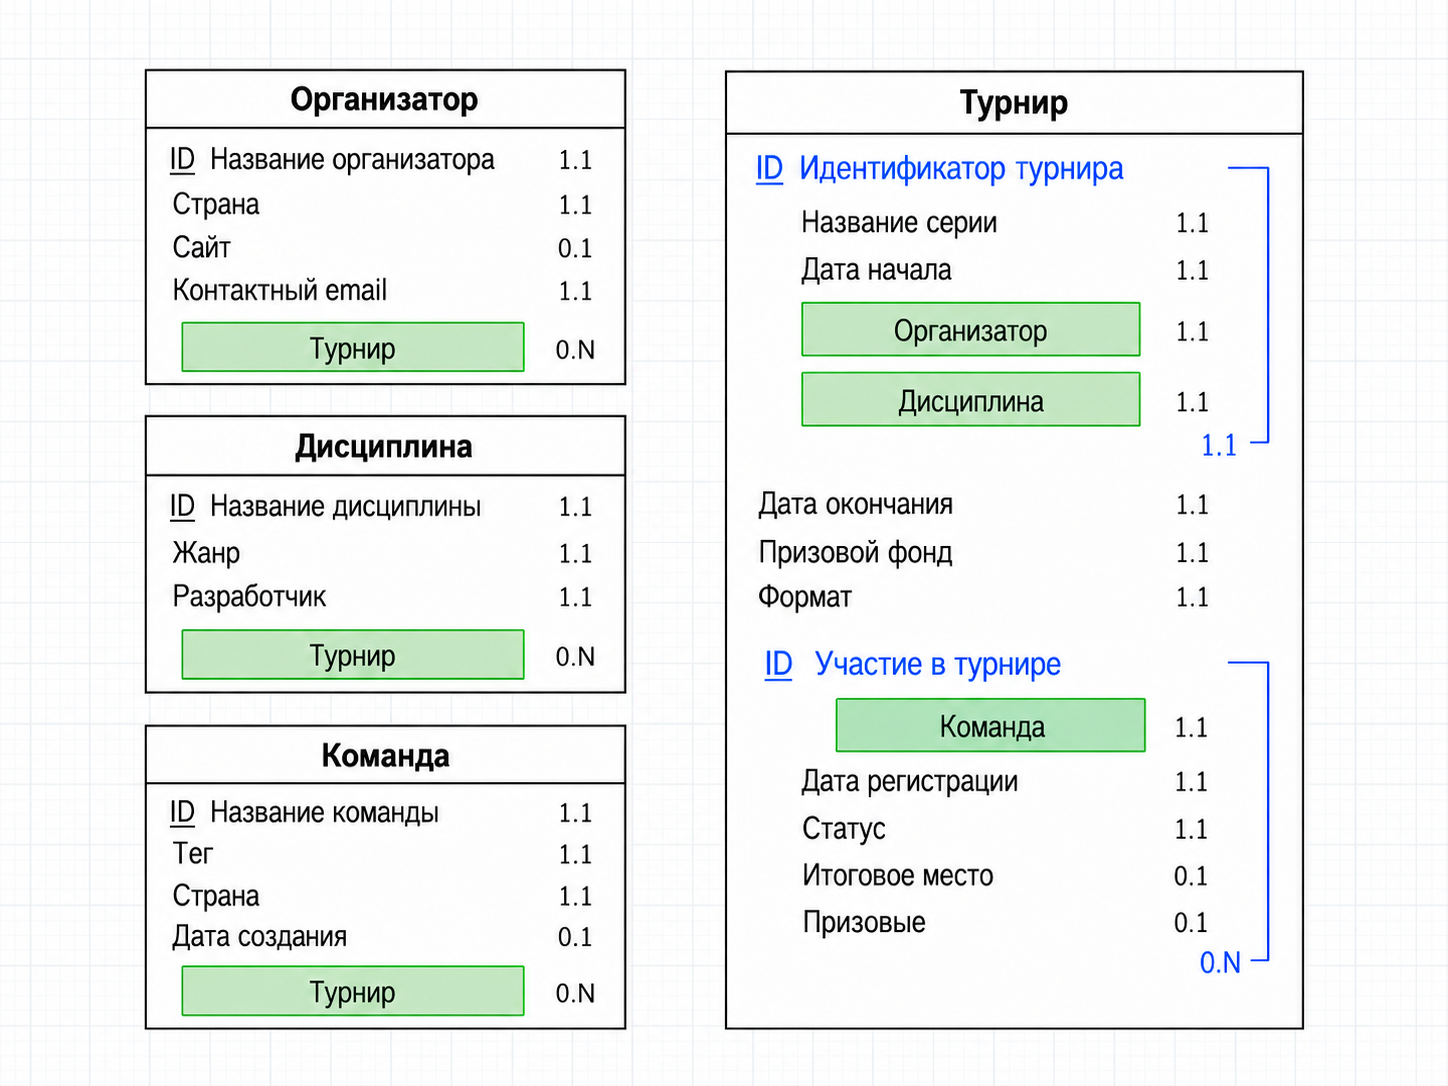
\includegraphics[width=0.83\textwidth]{labdb2.png}
  \caption{Модель семантических объектов}
  \label{fig:som-model}
\end{figure}


\clearpage
\subsection{Построение реляционной модели}
Объекты <<Организатор>>, <<Дисциплина>>, <<Команда>> и <<Турнир>> преобразованы в отношения. Многозначная группа <<Участие в турнире>> вынесена в отдельное отношение с внешними ключами на турнир и команду. Обратные объектные атрибуты реализуют те же связи и не требуют дополнительных таблиц.

Как и в работе № 3, для турнира и участия выбраны суррогатные PK, а исходная уникальность сохранена через составные AK. Полученная модель представлена на рисунке~\ref{fig:rel-model}.

\begin{figure}[H]
  \centering
  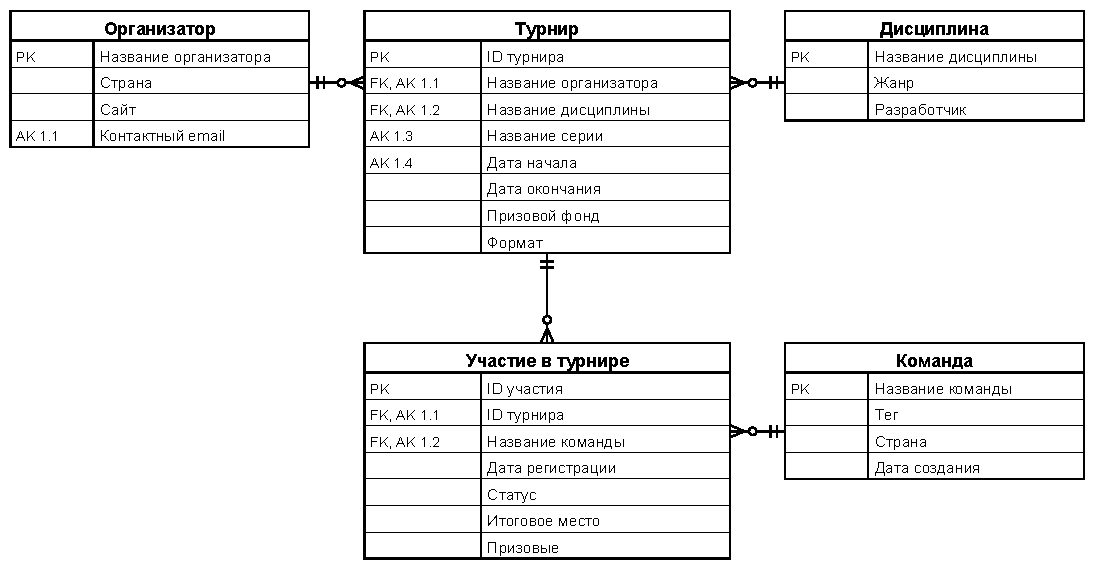
\includegraphics[width=\textwidth]{lab4_schema.pdf}
  \caption{Реляционная модель, полученная из модели семантических объектов}
  \label{fig:rel-model}
\end{figure}

\subsection{Сопоставление реляционных моделей}
Реляционные модели, полученные в лабораторных работах № 3 и № 4, совпадают по составу отношений, атрибутам, типам данных, ключам и кардинальностям связей. В работе № 3 отношение <<Участие в турнире>> получено из сущности ER-модели, а в работе № 4 --- из многозначной группы гибридного объекта <<Турнир>>.

Расхождений в структуре моделей не выявлено. Уточнено правило работы № 3: суррогатные <<ID турнира>> и <<ID участия>> являются неизменяемыми.

\end{document}
